\documentclass[xcolor={table}]{beamer}

% Packages
\usepackage[brazil]{babel}	
\usepackage[utf8]{inputenc}
\usepackage[T1]{fontenc}
\usepackage[scaled]{helvet}
\usepackage{amsthm}
\usepackage{ragged2e}
\usepackage{subfig}
\usepackage[table]{xcolor}
\usepackage{multicol}
\usepackage{multirow}
\usepackage{fancyvrb}
\usepackage{verbatim}
\usepackage{minted}

% Configuration for packages
\usemintedstyle{bw}

% Theme
\usetheme{Execushares}

% Title page configuration
\title{Laborator II: Suprascrierea Stivei. \textit{Shellcodes} I}
\subtitle{}
\author{Iosif George-Andrei}
\setcounter{showSlideNumbers}{1}

\begin{document}

    % Title page
    \setcounter{showProgressBar}{0}
	\setcounter{showSlideNumbers}{0}
	\frame{\titlepage}

    % Table of content
	\begin{frame}
		\frametitle{Tabelă de Conținut}\pause
		\begin{enumerate}[<+->]
			\item Suprascrierea Stivei
			\item \textit{Shellcodes} I
			\item Exemplu Concret
		\end{enumerate}
	\end{frame}

    % First section
	\setcounter{framenumber}{0}
	\setcounter{showProgressBar}{1}
	\setcounter{showSlideNumbers}{1}
	\section{Suprascrierea Stivei}

	\begin{frame}
		\frametitle{Suprascrierea \textit{Buffer}-ului}\pause
		\begin{itemize}[<+->]
			\item \textit{Buffer}: Zonă temporară de memorie, folosită la un moment dat pentru procesarea sau mutarea datelor.
			\item \textit{Suprascrierea Buffer-ului}: Scrierea într-un \textit{buffer} a unor date care depășesc limitele acestuia, suprascriind astfel zone de memorie vecine. Poate apărea la limbaje de programare care nu efectuează o verificare automată a limitelor zonelor de memorie în care se scrie (de exemplu, Assembly, C și C++).
		\end{itemize}
	\end{frame}
	
	\begin{frame}
		\frametitle{Categorii}\pause
		\begin{itemize}[<+->]
			\item În \textit{Stivă}: Zona de memorie suprascrisă aparține de stiva procesului, \textit{buffer}-ul fiind o variabilă locală.
			\item În \textit{\textit{Heap}}: Zona de memorie suprascrisă aparține de \textit{heap}, \textit{buffer}-ul fiind o variabilă alocată dinamic.
			\item \textit{La Nivel de Tip de Date}: Efectuarea de operațiuni care rezultă într-o valoare ce nu poate fi salvată într-un anumit tip de date. De exemplu, \mintinline{bash}{(char)(2 * 128)} e egal cu \mintinline{bash}{0}.
		\end{itemize}
	\end{frame}
	
	\begin{frame}
		\frametitle{Funcționare}\pause
		\centering
        \mintinline{bash}{sketch();}
	\end{frame}
	
	\begin{frame}
		\frametitle{Rezultatele Suprascrierii Stivei}\pause
		\begin{itemize}[<+->]
			\item Modificarea unor variabile
			    \begin{itemize}
        			\item Referințe către funcții
        			\item Canarii
        		\end{itemize}
        	\item Modificarea adreselor de retur
		\end{itemize}
	\end{frame}
	
	\begin{frame}
		\frametitle{Protecții}\pause
		\begin{itemize}[<+->]
			\item Impunerea unei lungimi maxime la copierea în \textit{buffer}
			\item Folosirea unor mecanisme de securitate impuse de compilator (canarii), la nivel de sistem de operare (Data Execution Prevention pe Windows) sau \textit{hardware} (bitul NX în intrările din tabelele de pagini ale procesorului)
		\end{itemize}
	\end{frame}
	
	% Second section
	\section{\textit{Shellcodes I}}

	\begin{frame}
		\frametitle{\textit{Shellcodes}}\pause
		\begin{itemize}[<+->]
			\item \textit{\textit{Shellcode}}: Secvență de coduri de operații folosită în exploatarea de programe pentru efectuarea unor sarcini (de obicei, deschiderea unui \textit{shell}).
			\item Scris în Assembly (recomandat datorită controlului mai mare), eventual în C (rezultatul depinde de compilator)
		\end{itemize}
	\end{frame}
	
	\begin{frame}
		\frametitle{Funcționare}\pause
		\centering
        \mintinline{bash}{sketch();}
	\end{frame}
	
	\begin{frame}
		\frametitle{Limitări în Scrierea \textit{Shellcode}-urilor}\pause
		\begin{itemize}[<+->]
			\item Dimensiunea \textit{buffer}-ului
			\item Posibilitatea interpretării unor octeți ca terminator de șir
			\item Detectabilitatea operațiunilor efectuate de către soluțiile de securitate
		\end{itemize}
	\end{frame}
	
	% Third section
	\section{Exerciții}
	
	\begin{frame}
		\frametitle{Exerciții}\pause
		\begin{enumerate}[<+->]
		    \item Suprascrierea Stivei
		    \item Crearea și Testarea unui \textit{Shellcode}
	    \end{enumerate}
	\end{frame}

	\begin{frame}
		\frametitle{Recomandări}\pause
		\begin{itemize}[<+->]
		    \item Folosiți comanda \mintinline{bash}{man} pentru a primi ajutor la rularea anumitor comenzi.
		    \item Folosiți \href{https://docs.pwntools.com/en/stable/}{documentația \mintinline{bash}{pwntools}} pentru a identifica metodele de care aveți nevoie.
	    \end{itemize}
	\end{frame}

    % Forth section
	\section{\textit{Exemplu Concret}}

	\begin{frame}
		\frametitle{RCE în Aplicația Client Steam}\pause
		\begin{itemize}[<+->]
		    \item \href{https://hackerone.com/reports/470520}{Vulnerabilitate raportată} în 2019, pe HackerOne
			\item Protocol proprietar pentru descoperirea serverelor de jocuri
			\item \textit{Fuzzing} efectuat pe protocol pentru a identifica un câmp vulnerabil, specific numelui de utilizator
			\item Suprascrierea \textit{buffer}-ului la nivel de stivă
			\item Folosirea unui \textit{shellcode} pentru lansarea \mintinline{bash}{cmd.exe}
			\item Depășirea unor limitări provocate de conversia Unicode a numelui (în acest caz, a \textit{payload}-ului) și de caracterele \mintinline{bash}{NULL}
		\end{itemize}
	\end{frame}
	
    % Fifth section
	\section{Recapitulare}

	\begin{frame}
		\frametitle{Recapitulare}\pause
		\begin{figure}
            \centering
            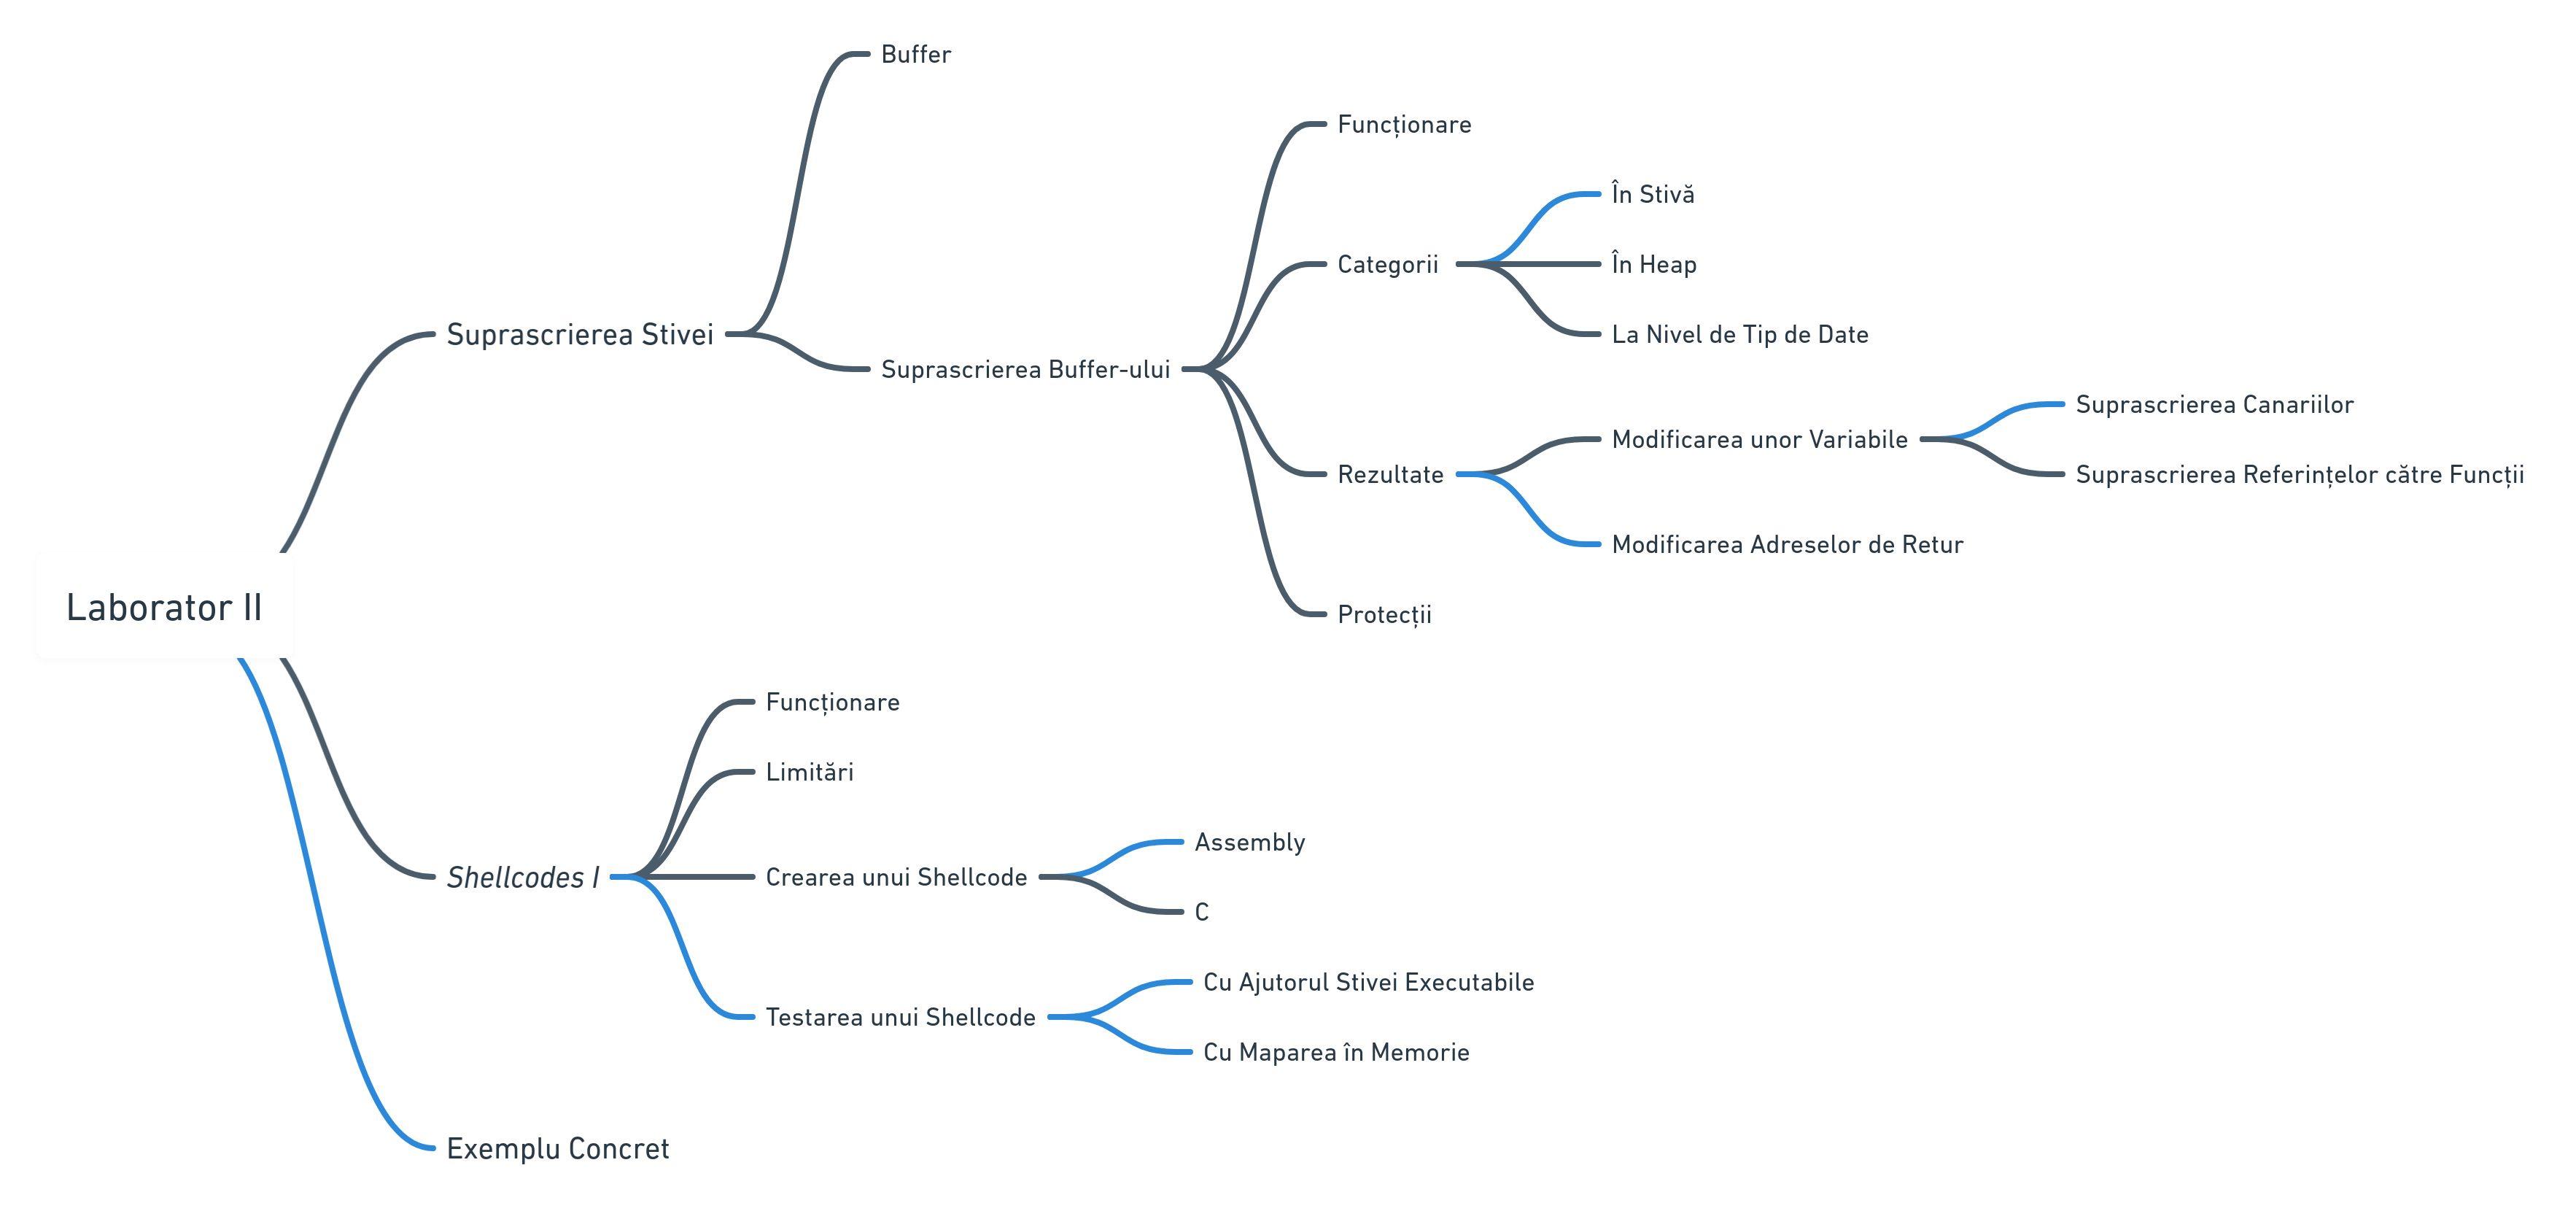
\includegraphics[width=11cm]{images/recap.png}
        \end{figure}
	\end{frame}

\end{document}